\documentclass{standalone}

\usepackage[T1]{fontenc}
\usepackage[utf8]{inputenc}
\usepackage{eulervm}
\usepackage{amsmath}
\usepackage{bm}
\usepackage{tikz}
\usepackage{environ}

\usetikzlibrary{fit}
\usetikzlibrary{patterns}
\usetikzlibrary{arrows}

\usepackage{color}

\definecolor{Comment}{RGB}{97,161,176}

\definecolor{btfGreen}{RGB}{51,160,44}
\definecolor{btfRed}{RGB}{190,60,90}

\definecolor{bleuUni}{RGB}{0, 157, 224}
\definecolor{marronUni}{RGB}{68, 58, 49}
\definecolor{grayMarronUni}{RGB}{60, 60, 60}
\definecolor{grayBleuUni}{RGB}{118, 118, 118}

\definecolor{bluecite}{HTML}{009DE0}

\definecolor{Paired-2}{RGB}{166,206,227}
\definecolor{Paired-1}{RGB}{31,120,180}
\definecolor{Paired-4}{RGB}{178,223,138}
\definecolor{Paired-3}{RGB}{51,160,44}
\definecolor{Paired-6}{RGB}{251,154,153}
\definecolor{Paired-5}{RGB}{227,26,28}
\definecolor{Paired-8}{RGB}{253,191,111}
\definecolor{Paired-7}{RGB}{255,127,0}
\definecolor{Paired-10}{RGB}{202,178,214}
\definecolor{Paired-9}{RGB}{106,61,154}
\definecolor{Paired-12}{RGB}{255,255,153}
\definecolor{Paired-11}{RGB}{177,89,40}
\definecolor{Accent-1}{RGB}{127,201,127}
\definecolor{Accent-2}{RGB}{190,174,212}
\definecolor{Accent-3}{RGB}{253,192,134}
\definecolor{Accent-4}{RGB}{255,255,153}
\definecolor{Accent-5}{RGB}{56,108,176}
\definecolor{Accent-6}{RGB}{240,2,127}
\definecolor{Accent-7}{RGB}{191,91,23}
\definecolor{Accent-8}{RGB}{102,102,102}
\definecolor{Spectral-1}{RGB}{158,1,66}
\definecolor{Spectral-2}{RGB}{213,62,79}
\definecolor{Spectral-3}{RGB}{244,109,67}
\definecolor{Spectral-4}{RGB}{253,174,97}
\definecolor{Spectral-5}{RGB}{254,224,139}
\definecolor{Spectral-6}{RGB}{255,255,191}
\definecolor{Spectral-7}{RGB}{230,245,152}
\definecolor{Spectral-8}{RGB}{171,221,164}
\definecolor{Spectral-9}{RGB}{102,194,165}
\definecolor{Spectral-10}{RGB}{50,136,189}
\definecolor{Spectral-11}{RGB}{94,79,162}
\definecolor{Set1-1}{RGB}{228,26,28}
\definecolor{Set1-2}{RGB}{55,126,184}
\definecolor{Set1-3}{RGB}{77,175,74}
\definecolor{Set1-4}{RGB}{152,78,163}
\definecolor{Set1-5}{RGB}{255,127,0}
\definecolor{Set1-6}{RGB}{255,255,51}
\definecolor{Set1-7}{RGB}{166,86,40}
\definecolor{Set1-8}{RGB}{247,129,191}
\definecolor{Set1-9}{RGB}{153,153,153}
\definecolor{Set2-1}{RGB}{102,194,165}
\definecolor{Set2-2}{RGB}{252,141,98}
\definecolor{Set2-3}{RGB}{141,160,203}
\definecolor{Set2-4}{RGB}{231,138,195}
\definecolor{Set2-5}{RGB}{166,216,84}
\definecolor{Set2-6}{RGB}{255,217,47}
\definecolor{Set2-7}{RGB}{229,196,148}
\definecolor{Set2-8}{RGB}{179,179,179}
\definecolor{Dark2-1}{RGB}{27,158,119}
\definecolor{Dark2-2}{RGB}{217,95,2}
\definecolor{Dark2-3}{RGB}{117,112,179}
\definecolor{Dark2-4}{RGB}{231,41,138}
\definecolor{Dark2-5}{RGB}{102,166,30}
\definecolor{Dark2-6}{RGB}{230,171,2}
\definecolor{Dark2-7}{RGB}{166,118,29}
\definecolor{Dark2-8}{RGB}{102,102,102}
\definecolor{Reds-1}{RGB}{255,245,240}
\definecolor{Reds-2}{RGB}{254,224,210}
\definecolor{Reds-3}{RGB}{252,187,161}
\definecolor{Reds-4}{RGB}{252,146,114}
\definecolor{Reds-5}{RGB}{251,106,74}
\definecolor{Reds-6}{RGB}{239,59,44}
\definecolor{Reds-7}{RGB}{203,24,29}
\definecolor{Reds-8}{RGB}{165,15,21}
\definecolor{Reds-9}{RGB}{103,0,13}
\definecolor{Greens-1}{RGB}{247,252,245}
\definecolor{Greens-2}{RGB}{229,245,224}
\definecolor{Greens-3}{RGB}{199,233,192}
\definecolor{Greens-4}{RGB}{161,217,155}
\definecolor{Greens-5}{RGB}{116,196,118}
\definecolor{Greens-6}{RGB}{65,171,93}
\definecolor{Greens-7}{RGB}{35,139,69}
\definecolor{Greens-8}{RGB}{0,109,44}
\definecolor{Greens-9}{RGB}{0,68,27}
\definecolor{Blues-1}{RGB}{247,251,255}
\definecolor{Blues-2}{RGB}{222,235,247}
\definecolor{Blues-3}{RGB}{198,219,239}
\definecolor{Blues-4}{RGB}{158,202,225}
\definecolor{Blues-5}{RGB}{107,174,214}
\definecolor{Blues-6}{RGB}{66,146,198}
\definecolor{Blues-7}{RGB}{33,113,181}
\definecolor{Blues-8}{RGB}{8,81,156}
\definecolor{Blues-9}{RGB}{8,48,107}


\begin{document}
  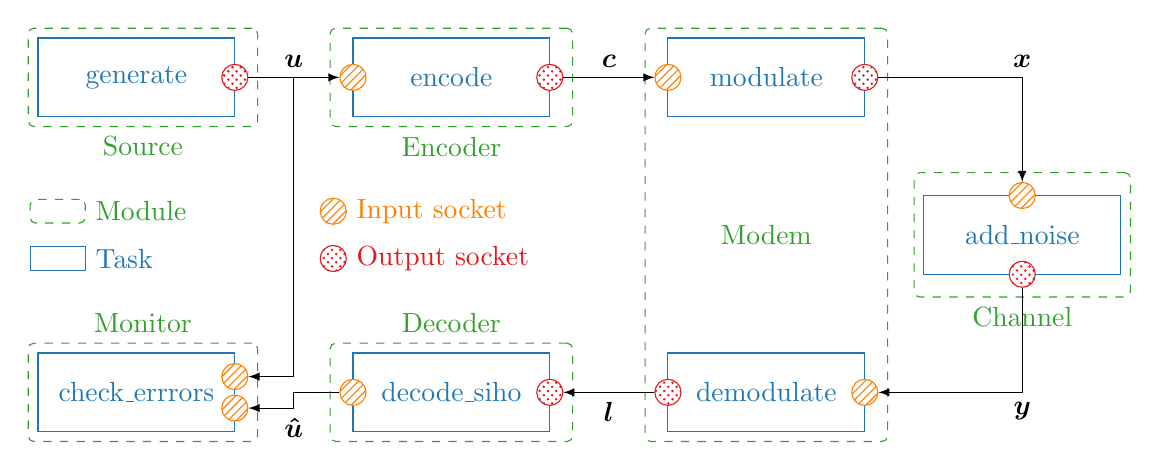
\begin{tikzpicture}%[scale=\tikzscale]
    \tikzset{ tsk/.style ={draw=Paired-1, rounded corners=0pt, minimum height=1cm, minimum width=2.5cm, text=Paired-1} }
    \tikzset{ mdl/.style ={draw=Paired-3, rounded corners=2pt,} }
    \tikzset{ sin/.style ={draw=Paired-7, circle, minimum width=0.3cm, text=black, preaction={fill=white}, pattern=north east lines, pattern color=Paired-7} }
    \tikzset{ sout/.style={draw=Paired-5, circle, minimum width=0.3cm, text=black, preaction={fill=white}, pattern=crosshatch dots, pattern color=Paired-5} }

    \node[tsk ] (src) at ( 0, 4) {generate};
    \node[sout] (src_so) at (0+1.25, 4) {};
    \node[tsk ] (enc) at ( 4, 4) {encode};
    \node[sin ] (enc_si) at (4-1.25, 4) {};
    \node[sout] (enc_so) at (4+1.25, 4) {};
    \node[tsk ] (mod) at ( 8, 4) {modulate};
    \node[sin ] (mod_si) at (8-1.25, 4) {};
    \node[sout] (mod_so) at (8+1.25, 4) {};
    \node[tsk ] (chn) at (11.25, 2) {add\_noise};
    \node[sin ] (chn_si) at (11.25, 2.5) {};
    \node[sout] (chn_so) at (11.25, 1.5) {};
    \node[tsk ] (dem) at ( 8, 0) {demodulate};
    \node[sout] (dem_so) at (8-1.25, 0) {};
    \node[sin ] (dem_si) at (8+1.25, 0) {};
    \node[tsk ] (dec) at ( 4, 0) {decode\_siho};
    \node[sin ] (dec_so) at (4-1.25, 0) {};
    \node[sout] (dec_si) at (4+1.25, 0) {};
    \node[tsk ] (mnt) at ( 0, 0) {check\_errrors};
    \node[sin ] (mnt_si1) at (0+1.25, +0.2) {};
    \node[sin ] (mnt_si2) at (0+1.25, -0.2) {};

    \node[mdl, label={[Paired-3]below:Source},  dashed, fit=(src) (src_so)] {};
    \node[mdl, label={[Paired-3]below:Encoder}, dashed, fit=(enc) (enc_si) (enc_so)] {};
    \node[mdl, label={[Paired-3]center:Modem},  dashed, fit=(mod) (dem) (mod_si) (mod_so) (dem_si) (dem_so)] {};
    \node[mdl, label={[Paired-3]below:Channel}, dashed, fit=(chn) (chn_si) (chn_so)] {};
    \node[mdl, label={[Paired-3]above:Decoder}, dashed, fit=(dec) (dec_si) (dec_so)] {};
    \node[mdl, label={[Paired-3]above:Monitor}, dashed, fit=(mnt) (mnt_si1) (mnt_si2)] {};

    \draw[->,>=latex] (src_so)               -- (enc_si)       node [midway, above] {$\bm{u}$};
    \draw[->,>=latex] (enc_so)               -- (mod_si)       node [midway, above] {$\bm{c}$};
    \draw[->,>=latex] (mod_so)               -| (chn_si)       node [midway, above] {$\bm{x}$};
    \draw[->,>=latex] (chn_so)               |- (dem_si)       node [midway, below] {$\bm{y}$};
    \draw[->,>=latex] (dem_so)               -- (dec_si)       node [midway, below] {$\bm{l}$};
    \draw[->,>=latex] (dec_so)      -- (2,0) |- (mnt_si2)      node [midway, below] {$\bm{\hat{u}}$};
    \draw[->,>=latex] (src_so.east) -- (2,4) |- (mnt_si1.east) node [midway, above] {};

    \node[draw=Paired-1, rounded corners=0pt,         minimum height=0.3cm, minimum width=0.7cm, text=Paired-1, label={[Paired-1]right:Task}         ] (l1) at (-1+0.0, 1.7) {};
    \node[draw=Paired-3, rounded corners=2pt, dashed, minimum height=0.3cm, minimum width=0.7cm, text=Paired-1, label={[Paired-3]right:Module}       ] (l2) at (-1+0.0, 2.3) {};
    \node[sout,                                                                                                 label={[Paired-5]right:Output socket}] (l3) at (-1+3.5, 1.7) {};
    \node[sin,                                                                                                  label={[Paired-7]right:Input socket} ] (l4) at (-1+3.5, 2.3) {};

  \end{tikzpicture}
\end{document}